\chapter{Moleküle}
Das einfachste Molekül H2 lässt sich mit dem Hamiltonian
\begin{align*}
	H &= -\frac{\hbar^2}{2m}\laplacian_{\mvec{r_1}} -\frac{\hbar^2}{2m}\laplacian_{\mvec{r_2}} -\frac{\hbar^2}{2M}\laplacian_{\mvec{R_1}} -\frac{\hbar^2}{2M}\laplacian_{\mvec{R_2}} \\
	&+ \frac{e^2}{4\pi\epsilon_0} \left(\frac{1}{|\mvec{r_1}-\mvec{r_2}|} + \frac{1}{|\mvec{R_1}-\mvec{R_2}|} -\frac{1}{|\mvec{R_1}-\mvec{r_1}|} - \frac{1}{|\mvec{R_1}-\mvec{r_2}|} - \frac{1}{|\mvec{R_2}-\mvec{r_1}|} - \frac{1}{|\mvec{R_2}-\mvec{r_2}|} \right)
\end{align*}
beschreiben.
Dieses Problem ist analytisch so nicht lösbar, schon gar nicht für kompliziertere Moleküle.

\section{Die Born-Oppenheimer-Näherung}
Bedenkt man allerdings, dass die Kerne viel schwerer als die Elektronen - demnach auch viel langsamer - sind, kann man folgenden Ansatz machen:
\begin{equation*}
	\mvec{R} =: \mvec{R_2}-\mvec{R_1} = \text{const}.
\end{equation*}
Das Molekül rotiert also nicht und wir halten in Gedanken $\mvec{R}$ fest.

Ein Näherungs-Hamiltonian besteht dann aus
\begin{equation*}
	H_\text{Kern} = -\frac{\hbar^2}{2M_r}\laplacian_{\mvec{R}} + V_\text{eff}(R).
\end{equation*}
Die elektronische Bindung des Moleküls gibt dann das $V_\text{eff}(R)$ vor.

\section{Bindungen}

\subsection{Die kovalente Bindung}
Entsteht durch Überlapp der Wellenfunktionen der einzelnen Atome.

\textbf{Beispiel: Wasserstoffmolekül}  Die Bindung zwischen zwei H-Atomen entsteht aus einem Gleichgewicht der Coulomb-Abstoßung der Kerne und der anziehenden Austauschwechselwirkung der Elektronen.
Das Symmetrisierungspostulat der QM schreibt nun eine Verschränkung der Wellenfunktionen
\begin{align*}
	\psi_\text{s/a} = \varPsi(\mvec{x_1})\varphi(\mvec{x_2}) \pm \varphi(\mvec{x_1})\varPsi(\mvec{x_2})
\end{align*}
vor.
Es existieren also zwei Zustände: der bindende (sym.) und der antibindende (antisym.) Zustand.

Beim bindenden Zustand haben die Elektronen aufgrund des additiven Überlapps der Wellenfunktionen die größte Aufenthaltswahrscheinlichkeit zwischen den Kernen des Moleküls und schirmen somit die Coulomb-Abstoßung der Kerne teilweise ab.
Beim antibindenden Zustand jedoch, weisen die Elektronen keine Aufenthaltswahrscheinlichkeit zwischen den Kernen auf und es kommt zur Abstoßung der Atome.

\subsection{Van-der-Waals-Wechselwirkungen}
Edelgasatome (z.B. He) besitzen bereits eine sehr stabile $\el$-Konfiguration, daher ist keine kovalente Bindung möglich.
Jedoch können polarisierbare Moleküle induzierte Dipol-Dipol-Wechselwirkungen ausführen.

Um diese Bindung zu beschreiben, wird oft ein phänomenlogisches \textbf{Lennard-Jones-Potenzial}
\begin{equation*}
	V_\text{eff}(R) = 4\varepsilon\left( -\left(\frac{\sigma}{R}\right)^6 + \left(\frac{\sigma}{R}\right)^{12}\right)
\end{equation*}
angesetzt.

\subsection{Ionische Bindung}
Betrachten wir nun die Bindung zweier verschiedener Atome, z.B. Na und Cl.
Gibt das Na ein $\el$ an das Cl ab, so weisen beide abgeschlossene Schalen auf (energieärmster Zustand) und es entstehen ein Na+ und Cl- Ion.
Diese ziehen sich aufgrund der Coulomb-WW an.

\section{Molekülschwingungen}
\begin{figure}
	\centering
	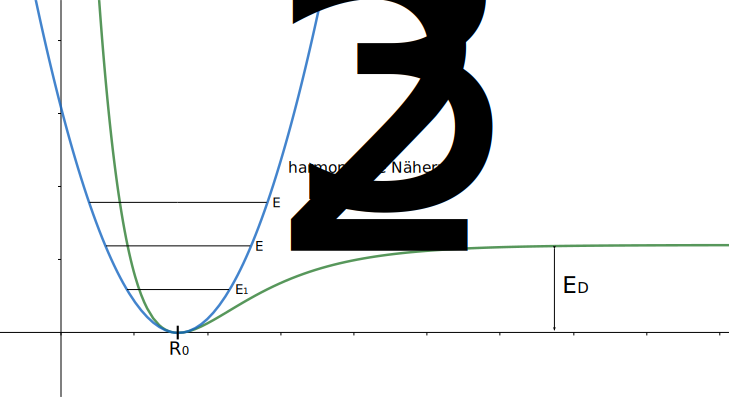
\includegraphics[width=.5\textwidth]{./img/harm_approx.pdf}
	\caption{Das \textsc{Morse}-Potenzial und die harmonische Näherung}
	\label{fig:harmapprox}
\end{figure}
Eine Molekülschwingung ist die periodische Bewegung von benachbarten Atomen innerhalb eines Moleküls.
Betrachten wir ein zweiatomiges Molekül, so wird das elektronische Potential in Abhängigkeit vom Kernbindungsabstand $R$ beschrieben durch das \textbf{Morse-Potenzial}
\begin{equation*}
	V_\text{M} = E_\text{D}\left(1 - e^{-a(R-R_0)}\right)^2.
\end{equation*}
Um das Problem leichter lösen zu können, machen wir (wie immer) eine harmonische Näherung
\begin{equation*}
	V_\text{M} \approx E_\text{D}a^2\left(R-R_0\right)^2.
\end{equation*}
Wie beim harmonischen Oszillator ergeben sich nun quantisierte Energieniveaus (siehe \autoref{fig:harmapprox}).

\begin{equation*}
	E_\nu = \hbar\Omega\left(\nu+\frac{1}{2}\right) - \frac{\hbar^2\Omega^2}{4E_\text{D}}\left(\nu+\frac{1}{2}\right)^2.
\end{equation*}
Atome können also zu Molekülschwingungen angeregt werden (z.B. durch Photonen).

\section{Molekülrotationen}
Im einfachsten Fall kann die Rotation eines Moleküles durch einen starren Rotor mit der Rotationsenergie
\begin{equation*}
	E_\text{rot} = \frac{|\mvec{L}|^2}{2I} = \frac{\hbar^2}{2I}J(J+1)
\end{equation*}
beschrieben werden, wobei $I$ sein Trägheitsmoment bezüglich der Rotationsachse ist.
